\documentclass[parskip=half-,DIV=12,twoside=semi, 12pt]{scrartcl}
% \usepackage{showframe}
\usepackage[french]{babel}
\usepackage[T1]{fontenc}
\usepackage[utf8]{inputenc}
\usepackage{microtype}
\usepackage[sfmath, light]{kpfonts} %police
\renewcommand{\familydefault}{\sfdefault}
\usepackage{mathtools}
\newcommand{\abs}[1]{\mid#1\mid}
\usepackage{fontawesome5}
\usepackage{multicol}
\usepackage{enumitem}
\SetEnumitemKey{cols}{
itemsep = 1\itemsep,
parsep = 1\parsep,
before = \raggedcolumns\begin{multicols}{#1},
after = \end{multicols}}
\setlist[enumerate]{label=\textbf{\alph*)}}
\newlist{qcm}{itemize}{1}
\setlist[qcm]{label=\faIcon[regular]{square}, cols=3}

\usepackage{eurosym} % \EUR{8} --> 8 €
\usepackage{multicol}
\usepackage[locale=FR]{siunitx}
\DeclareSIUnit{\sieuro}{\mbox{\euro}}
\usepackage{tikz}
\usetikzlibrary{babel, patterns, matrix}
\usepackage{tkz-base}
\usepackage{tkz-euclide}
\usepackage{tikzscale}
\usepackage{pgfplots}
\pgfplotsset{width=15cm,compat=1.9}
\usepackage{graphicx}
\usepackage{tabularray}
\NewColumnType{C}[1][]{Q[c,co=1,#1]}
\usepackage{tcolorbox}
\tcbuselibrary{skins, xparse}
\usepackage{ulem}
\usepackage[use-aux, use-files]{xsim}

\DeclareExerciseEnvironmentTemplate{interrogation}
{%
    \colorbox{black}{\color{white}\bfseries\GetExerciseProperty{counter}}
    % {\bfseries\XSIMmixedcase{\GetExerciseName}\nobreakspace\GetExerciseProperty{counter}.}%
    \GetExercisePropertyT{points}{\marginpar{\qquad/\bfseries\PropertyValue}}
    \GetExercisePropertyT{subtitle}{\normalfont\itshape\PropertyValue}
}%
{\bigbreak}

% Mes environnements
\DeclareExerciseType{connaitre}{
exercise-env = connaitre ,
solution-env = solconnaitre ,
exercise-name = \XSIMtranslate{question} ,
exercises-name = \XSIMtranslate{questions} ,
solution-name = \XSIMtranslate{solution} ,
solutions-name = \XSIMtranslate{solutions} ,
exercise-template = interrogation ,
solution-template = interrogation ,
exercise-heading = \subsection* ,
solution-heading = \subsection*,
counter = exercise
}
\DeclareExerciseType{appliquer}{
exercise-env = appliquer ,
solution-env = solappliquer ,
exercise-name = \XSIMtranslate{question} ,
exercises-name = \XSIMtranslate{questions} ,
solution-name = \XSIMtranslate{solution} ,
solutions-name = \XSIMtranslate{solutions} ,
exercise-template = interrogation ,
solution-template = interrogation ,
exercise-heading = \subsection* ,
solution-heading = \subsection*,
counter = exercise
}
\DeclareExerciseType{transferer}{
exercise-env = transferer ,
solution-env = soltransferer ,
exercise-name = \XSIMtranslate{question} ,
exercises-name = \XSIMtranslate{questions} ,
solution-name = \XSIMtranslate{solution} ,
solutions-name = \XSIMtranslate{solutions} ,
exercise-template = interrogation ,
solution-template = interrogation ,
exercise-heading = \subsection* ,
solution-heading = \subsection*,
counter = exercise
}

\xsimsetup{
    path=xsim,
    exercise/template = interrogation,
    solution/template = interrogation,
    blank/style=\dotuline{#1},
}

\newcommand{\figcolor}{white}
\newcommand{\Titre}{TJF - Les inéquations}
\newcommand{\Date}{Vendredi 25 novembre 2022}
\newcommand{\Classe}{}

% \usepackage{scrlayer-scrpage}
% \setlength{\headheight}{50pt}
% \lohead{Nom :\smallbreak Prénom :\smallbreak Classe : \Classe}
% \rohead{\No~\fbox{\phantom{XX}}\smallbreak ~\smallbreak \Date}

\setlength{\textheight}{700pt}
\newcounter{l}
\setcounter{l}{1}
\begin{document}
\raggedbottom
\pagestyle{empty}
%%%%%%%%%%%%%%%%%%%%%%%%%%%%%%%%%%%%%%%%%%%%%%%%%
% ENTETE
%%%%%%%%%%%%%%%%%%%%%%%%%%%%%%%%%%%%%%%%%%%%%%%%%

\includegraphics[width=\linewidth]{img/entete.pdf}
\vspace{\smallskipamount}
\begin{tblr}{%
        width=\textwidth,%
        colspec={|XXX|},%
        cell{1}{1} = {r=1, c=3}{c,font=\bfseries\Huge},%
        cell{2}{1}= {r=1, c=3}{c,font=\bfseries\Large},%
        cell{5}{1}={r=1,c=2}{l},
        cell{5}{3}={r=4,c=1}{r},
        cell{6}{1}={r=1,c=3}{l},%
        cell{7}{1}={r=1,c=3}{l},%
        cell{8}{1}={r=1,c=3}{l},%
        row{9} = {c},
        cell{10}{1}={r=1,c=3}{r},%
        rowsep=1ex%
    }%
    \hline
    % cell1
    Examen de mathématiques                 &   &                               \\
    % cell2
    Juin 2023                               &   &                               \\
    \hline
    % cell3
    Nom :                                   &   & Classe :                      \\
    % cell4
    Prénom :                                &   & Numéro :                      \\
    \hline
    % cell5
    Professeur : Baudoin, Debroux, Janssens &   &                               \\
    % cell6
    Date et heure : Mercredi 28 juin 2023 de 8 h 20 à 10 h 30                   \\
    % cell7
    Matériel autorisé : Équerre multifonction, crayons de couleur, calculatrice \\
    % cell8
    Matériel à distribuer : aucun                                               \\
    \hline
    % cell9
    C1 : \qquad/\TotalExerciseTypeGoal{connaitre}{points}{}{}
                                            &
    C2 : \qquad/\TotalExerciseTypeGoal{appliquer}{points}{}{}
                                            &
    C3 : \qquad/\TotalExerciseTypeGoal{transferer}{points}{}{}
    \\
    Total :
    \qquad/\TotalExerciseGoal{points}{}{}
    \quad\faIcon{arrow-right}\quad
    \qquad/30                               &   &                               \\
    \hline
\end{tblr}%
\vspace{\smallskipamount}
\begin{scriptsize}%
    Rue de linthout, 30 - 1030 Bruxelles%
\end{scriptsize}%
\medbreak
Quelques conseils pour réussir ton examen :
\begin{enumerate}[itemsep=0.5cm, label=$\bullet$]
    \item Toutes tes réponses doivent être soignées et écrites sur ce questionnaire.
    \item Ne te précipite pas. Commence par identifier ce que tu dois faire en lisant correctement et attentivement l'énoncé.
    \item S'il y a plusieurs questions dans un énoncé, veille à répondre à chacune d'entre elles.
    \item Utilise le vocabulaire adéquat.
    \item Veille à faire tes constructions au crayon et proprement.
    \item Commence par répondre à ce que tu maitrises, et reviens ensuite sur les questions qui te demandent plus de temps.
    \item Prends le temps de bien te relire !
\end{enumerate}
\vfill
\begin{flushright}
    Bon examen !
\end{flushright}
\cleardoublepage
\setcounter{page}{1}
\pagestyle{plain}
%%%%%%%%%%%%%%%%%%%%%%%%%%%%%%%%%%%%%%%%%%%%%%%%%
% CONTENU %
%%%%%%%%%%%%%%%%%%%%%%%%%%%%%%%%%%%%%%%%%%%%%%%%%
\begin{connaitre}[points=5]
    %FIXME: Tout est faux. On peut mettre corrige les proposition ci-dessous. C'est plus simple à corriger.
    Vrai ou faux? Justifie dans tous les cas.
    \begin{enumerate}[itemsep=2cm, after=\vspace*{2cm}]
        \item 24 est un diviseur de 12.
        \item \(-3\) est un nombre naturel.
        \item Dans un repère cartésien, l'axe vertical s'appelle l'axe des abscisses.
        \item Pour calculer \SI{7}{\%} d'un nombre, on le multiplie par 0,7.
        \item Le nombre de dents d'un enfant est proportionnel à son âge.
    \end{enumerate}
\end{connaitre}
%%%%%%%%%%%%%%%%%%%%%%%%%%%%%%%%%%%%%%%%%%%%%%%%%%
\begin{connaitre}[points=6]
    Coche la ou les bonnes réponses.
    \begin{enumerate}
        \item Quels sont les nombres qui sont premiers ?
              \begin{qcm}
                  \item 12
                  \item 1
                  \item 7
              \end{qcm}
        \item Quel est l'élément caractéristique d'une translation ?
              \begin{qcm}
                  \item Le vecteur
                  \item L'axe de symétrie
                  \item Le centre de symétrie
              \end{qcm}
        \item Quels sont les nombres carrés ?
              \begin{qcm}
                  \item 30
                  \item 25
                  \item 50
              \end{qcm}
        \item Comment s'appelle une droite qui partage un segment en deux parts égales, perpendiculairement ?
              \begin{qcm}
                  \item Une médiane
                  \item Une médiatrice
                  \item Une bissectrice
              \end{qcm}
              \newpage
        \item Quel nom donne-t-on à un triangle ayant trois côtés de longueurs différentes ?
              \begin{qcm}
                  \item Isocèle
                  \item Équilatéral
                  \item Scalène
              \end{qcm}
        \item \(\widehat{A}\) et \(\widehat{B}\) sont deux angles supplémentaires. Quelle égalité traduit cette proposition ?
              \begin{qcm}
                  \item \(\abs{\widehat{A}} + \abs{\widehat{B}} = \ang{180}\)
                  \item \(\abs{\widehat{A}} +  \abs{\widehat{B}} = \ang{90}\)
                  \item \(\abs{\widehat{A}} \cdot \abs{\widehat{B}} = \ang{180}\)
              \end{qcm}
        \item Que vaut le produit de 3 par \(-2\) ?
              \begin{qcm}
                  \item 6
                  \item 1
                  \item \(-6\)
              \end{qcm}
    \end{enumerate}
\end{connaitre}
%%%%%%%%%%%%%%%%%%%%%%%%%%%%%%%%%%%%%%%%%%%%%%%%%%
\begin{connaitre}[points=1]
    Quelle est la propriété illustrée par l'égalité suivante ?

    \hfil \(13+82 = 82 + 13\) \hfil \blank[scale=2]{commutativité}
\end{connaitre}
%%%%%%%%%%%%%%%%%%%%%%%%%%%%%%%%%%%%%%%%%%%%%%%%%%
\begin{connaitre}[points=1]
    %FIXME: Est-ce qu'on imposerait pas le nombre à décomposer ? Pour une correction plus facile.
    Calcule à l'aide de la distributivité simple. Laisse ta démarche visible.
    \[49 \cdot 8=\]
\end{connaitre}
%%%%%%%%%%%%%%%%%%%%%%%%%%%%%%%%%%%%%%%%%%%%%%%%%%
\begin{connaitre}[points=3]
    Donne la définition des concepts suivants. Sois précis.
    \begin{enumerate}[itemsep=2cm, after=\vspace*{2cm}]
        \item Valeur absolue.
        \item Bissectrice.
        \item Isométrie.
    \end{enumerate}
\end{connaitre}
%%%%%%%%%%%%%%%%%%%%%%%%%%%%%%%%%%%%%%%%%%%%%%%%%%
\begin{connaitre}[points=1]
    Donne un exemple de deux nombres opposés.
    \vspace*{2cm}
\end{connaitre}
%%%%%%%%%%%%%%%%%%%%%%%%%%%%%%%%%%%%%%%%%%%%%%%%%%
\begin{connaitre}[points=2]
    Code ou décode les expressions mathématiques ci-dessous.
    \begin{enumerate}[itemsep=1cm, after=\vspace*{1cm}]
        \item \((5-3)^2\)
        \item La somme de 5 et de l'opposé de 3
    \end{enumerate}
\end{connaitre}
%%%%%%%%%%%%%%%%%%%%%%%%%%%%%%%%%%%%%%%%%%%%%%%%%%
%FIXME: pourquoi ne pas mettre avec la précédente ? C'est aussi une question de codage, décodage.
\begin{connaitre}[points=1]
    Traduis par une phrase la notation suivante : \(S_{PM}(ABC) = A'B'C'\). \vspace*{2cm}
\end{connaitre}
%%%%%%%%%%%%%%%%%%%%%%%%%%%%%%%%%%%%%%%%%%%%%%%%%%
\begin{appliquer}[points=2]
    Effectue.
    \begin{enumerate}[cols=2]
        \item \((-3)^2 =\)
        \item \(-5 \cdot 2 = \)
    \end{enumerate}
\end{appliquer}
%%%%%%%%%%%%%%%%%%%%%%%%%%%%%%%%%%%%%%%%%%%%%%%%%%
\begin{appliquer}[points=5]
    Effectue. Laisse tes étapes visibles.
    \begin{enumerate}[cols=2, itemsep=2cm]
        \item \(8+(4-2)^2\cdot 3=\)
        \item \(5-2+4\cdot (3+2)=\)
        \item \(-2-(-7)\cdot 5=\)
        \item \(-5\cdot 3\cdot 0=\)
        \item \(-8 + 7 -(7+(-9))=\)
    \end{enumerate}
    \vspace*{2cm}
\end{appliquer}
%%%%%%%%%%%%%%%%%%%%%%%%%%%%%%%%%%%%%%%%%%%%%%%%%
%%%%%%%%%%%%%%%%%%%%%%%%%%%%%%%%%%%%%%%%%%%%%%%%%%
\begin{appliquer}[points=11]
    Effectue. Si tu ne peux pas réduire l'expression, recopie-la.
    %FIXME: Trop peu de place pour mettre sur deux colonnes, on peut utiliser task mais ...
    \begin{enumerate}[itemsep=2cm]
        \item \(8u-4+3u=\)
        \item \(m\cdot m \cdot m =\)
        \item \(-2a(3a-5b)=\)
        \item \(4x\cdot 3p + 2p \cdot 7x=\)
        \item \(t-(3t-6) + 3t=\)
        \item \(a^2 - a=\)
        \item \(4a\cdot 5a^2b + 2(5a^3b -7)=\)
        \item \(3x + 2x(3-x) + (2x^2-7x)=\)
        \item \(3a \cdot (a+2)=\)
        \item \(2x \cdot (-3y) - 6x + 7y=\)
        \item \(6x \cdot (-3xy) + 7x^2 \cdot 2y=\)
    \end{enumerate}
    \vspace*{2cm}
\end{appliquer}
%%%%%%%%%%%%%%%%%%%%%%%%%%%%%%%%%%%%%%%%%%%%%%%%%
%%%%%%%%%%%%%%%%%%%%%%%%%%%%%%%%%%%%%%%%%%%%%%%%%%
\begin{appliquer}[points=4]
    Complète les pointillés.
    \begin{enumerate}[cols=2]
        \item \(10a\cdot \blank[width=1cm]{} = 30a\)
        \item \(a + \blank[width=1cm]{} = 2a\)
        \item \(x \cdot \blank[width=1cm]{} = x^2\)
        \item \(-(8x+6y)- (\blank[width=1cm]{} - \blank[width=1cm]{} ) = 10x + 2y\)
    \end{enumerate}
\end{appliquer}
%%%%%%%%%%%%%%%%%%%%%%%%%%%%%%%%%%%%%%%%%%%%%%%%%
%%%%%%%%%%%%%%%%%%%%%%%%%%%%%%%%%%%%%%%%%%%%%%%%%%
%TODO: Flèche sur le tableau
\begin{appliquer}[points=4]
    Complète les tableaux de proportionnalité suivant. Indique ensuite le coefficient de proportionnalité relatif à chaque tableau.
    \begin{center}
        \begin{tblr}{
                hlines,
                vlines,
                columns={2cm, c},
                rows={1cm,m},
            }
            x & 8 & 27 &     & 30 &    \\
            y &   &    & 6,3 & 15 & 30
        \end{tblr}
    \end{center}

    \begin{center}
        \begin{tblr}{
                hlines,
                vlines,
                columns={2cm, c},
                rows={1cm,m},
            }
            x & 2 & 5 & 9  & 10 &    \\
            y &   &   & 27 &    & 33
        \end{tblr}
    \end{center}

\end{appliquer}
%%%%%%%%%%%%%%%%%%%%%%%%%%%%%%%%%%%%%%%%%%%%%%%%%
%%%%%%%%%%%%%%%%%%%%%%%%%%%%%%%%%%%%%%%%%%%%%%%%%%
\begin{appliquer}[points=2]
    Trace en vert la hauteur issue de \(A \)et en bleu la médiane relative à \([AB]\). Code ton dessin.
    \begin{center}
        
\includegraphics[width=10cm]{tikz/triangle.tikz}
    \end{center}
\end{appliquer}
%%%%%%%%%%%%%%%%%%%%%%%%%%%%%%%%%%%%%%%%%%%%%%%%%
%%%%%%%%%%%%%%%%%%%%%%%%%%%%%%%%%%%%%%%%%%%%%%%%%%
\begin{appliquer}[points=7]
    Complète les cases vides du tableau par le(s) mot(s) adéquat(s).
    \begin{center}
        \begin{tblr}{
                hlines,
                vlines,
                columns={4.5cm, c},
                rows={1.5cm,m},
                row{1}={gray!40, font=\bfseries},
            }
            Je suis \dots              & Si j'avais aussi \dots          & Je serais \dots \\
            Un parallélogramme         & les diagonales de même longueur &                 \\
            Un parallélogramme         & au moins un angle droit         &                 \\
            Un quadrilatère quelconque &                                 & un trapèze      \\
            Un parallélogramme         &                                 & un losange      \\
                                       & les diagonales de même longueur & un carré        \\
                                       & les angles droits               & un carré        \\
                                       & les côtés de même longueur      & un carré        \\
        \end{tblr}
    \end{center}

\end{appliquer}
%%%%%%%%%%%%%%%%%%%%%%%%%%%%%%%%%%%%%%%%%%%%%%%%%
%%%%%%%%%%%%%%%%%%%%%%%%%%%%%%%%%%%%%%%%%%%%%%%%%%
\begin{appliquer}[points=2]
    Factorise en mettant en évidence.
    \begin{enumerate}[cols=2]
        \item \(ab+6a^2=\)
        \item \(6a^3b^6 - 9a^2b^3=\)
    \end{enumerate}
\end{appliquer}
%%%%%%%%%%%%%%%%%%%%%%%%%%%%%%%%%%%%%%%%%%%%%%%%%
%%%%%%%%%%%%%%%%%%%%%%%%%%%%%%%%%%%%%%%%%%%%%%%%%%
\begin{appliquer}[points=2]
    Trace un rectangle \(EXAM\) si tu sais que ses diagonales mesurent \SI{5}{cm} et que l'angle aigu entre ses diagonales est de \ang{40}.
\end{appliquer}
\newpage
%%%%%%%%%%%%%%%%%%%%%%%%%%%%%%%%%%%%%%%%%%%%%%%%%
%%%%%%%%%%%%%%%%%%%%%%%%%%%%%%%%%%%%%%%%%%%%%%%%%%
\begin{appliquer}[points=3]
    Voici un repère cartésien.
    \begin{center}
        
\includegraphics{tikz/repere.tikz}
    \end{center}
    % 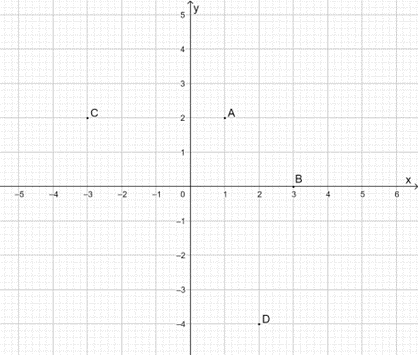
\includegraphics{img/graphe.png}
    \begin{enumerate}
        \item Écris les coordonnées des points suivants. \\
              \(A(\blank[width=1cm]{}; \blank[width=1cm]{})\) \hfill \(B(\blank[width=1cm]{}; \blank[width=1cm]{})\) \hfill  \(C(\blank[width=1cm]{}; \blank[width=1cm]{})\) \hfill  \(D(\blank[width=1cm]{}; \blank[width=1cm]{})\)
        \item Place le point \(X\) tel que \(X(-5;-2)\)
        \item Complète les phrases suivantes par \(A, B, C\) ou \(D\).
              %\begin{enumitem} \TODO: enumitem (TITI : je ne comprends pas)
        \item Mon ordonnée vaut le double de mon abscisse, je suis le point \dotfill
        \item Nous avons la même ordonnée, nous sommes les points \dotfill
              %\end{enumitem}
    \end{enumerate}
\end{appliquer}
%%%%%%%%%%%%%%%%%%%%%%%%%%%%%%%%%%%%%%%%%%%%%%%%%
%%%%%%%%%%%%%%%%%%%%%%%%%%%%%%%%%%%%%%%%%%%%%%%%%%
\begin{appliquer}[points=2]
    Réalise la construction demandée. Veille à laisser tes constructions visibles et à faire preuve de précision et de soin.
    \begin{center}
        \(t_{\overrightarrow{XY}}(ABCD)=A'B'C'D'\)

        \includegraphics[width=.5\linewidth]{tikz/translation.tikz}
    \end{center}
\end{appliquer}
%%%%%%%%%%%%%%%%%%%%%%%%%%%%%%%%%%%%%%%%%%%%%%%%%
%%%%%%%%%%%%%%%%%%%%%%%%%%%%%%%%%%%%%%%%%%%%%%%%%%
\begin{appliquer}[points=3]
    Observe la figure dans son ensemble, puis suis les consignes ci-dessous.
    Pour chaque ligne du tableau :
    \begin{enumerate}
        \item Dans la première colonne, indique s'il s'agit d'une translation (T), d'une symétrie centrale (SC) ou d'une symétrie orthogonale (SO).
        \item Dans la deuxième colonne, cite l'élément caractéristique de cette transformation du plan.
    \end{enumerate}
    \begin{center}
        \includegraphics[width=.5\linewidth]{tikz/figure001.tikz}
    \end{center}
    \begin{center}
        \begin{tblr}{
                hlines,
                vlines,
                hline{1}={1}{white},
                vline{1}={1}{white},
                columns={4cm, c},
                rows={1cm,m},
                row{1}={gray!40, font=\bfseries},
                column{1}={gray!40, font=\bfseries},
                cell{1}{1}={white}
            }
                     & Isométrie & Élément caractéristique \\
            De 2 à 3 &           &                         \\
            De 3 à 4 &           &                         \\
            De 1 à 4 &           &                         \\
        \end{tblr}
    \end{center}

\end{appliquer}
%%%%%%%%%%%%%%%%%%%%%%%%%%%%%%%%%%%%%%%%%%%%%%%%%
%%%%%%%%%%%%%%%%%%%%%%%%%%%%%%%%%%%%%%%%%%%%%%%%%%
\begin{appliquer}[points=3]
    Construis ce trapèze avec les dimensions réelles.

    \includegraphics[width=5cm]{tikz/figure002.tikz}
\end{appliquer}
\newpage
%%%%%%%%%%%%%%%%%%%%%%%%%%%%%%%%%%%%%%%%%%%%%%%%%%
%%%%%%%%%%%%%%%%%%%%%%%%%%%%%%%%%%%%%%%%%%%%%%%%%%
\begin{transferer}[points=3]
    Un automobiliste met du temps à payer son amende pour excès de vitesse de \SI{9}{\sieuro}. Il doit donc payer l'amende augmentée de 10\%.\\
    Quel est le nouveau montant que l'automobiliste va payer ? Laisse ta démarche visible.\vspace*{2cm}
\end{transferer}
%%%%%%%%%%%%%%%%%%%%%%%%%%%%%%%%%%%%%%%%%%%%%%%%%
%%%%%%%%%%%%%%%%%%%%%%%%%%%%%%%%%%%%%%%%%%%%%%%%%%
\begin{transferer}[points=4]
    Dans le cadre d'une exposition, un artiste a empilé des canettes. L'illustration ci-dessous montre les trois rangées du haut du montage.

    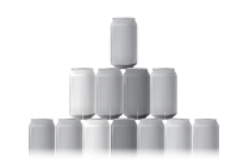
\includegraphics{img/cannettes.png}

    \begin{enumerate}[itemsep=1cm, after=\vspace*{
        1cm
    }]
        \item Complète ce tableau.
              \begin{center}
                  \begin{tblr}{
                          hlines,
                          vlines,
                          colspec={l*{6}{X[c]}},
                          rows={1cm,m},
                          column{1}={gray!40, font=\bfseries},
                      }
                      Numéro de la rangée & 1 & 2 & 3 & 4 & 5 & 6  \\
                      Nombre de cannettes & 1 & 4 & 7 &   &   & 16
                  \end{tblr}
              \end{center}
              \item Propose une formule qui permet de calculer le nombre de canettes \(c\) nécessaire en fonction du numéro de la rangée \(n\).
              \item Détermine le numéro de la rangée qui comporte 31 canettes en utilisant ta formule.
              \item Détermine le nombre de canettes de la 9\ieme{} rangée en utilisant ta formule.
    \end{enumerate}
\end{transferer}
%%%%%%%%%%%%%%%%%%%%%%%%%%%%%%%%%%%%%%%%%%%%%%%%%%
%%%%%%%%%%%%%%%%%%%%%%%%%%%%%%%%%%%%%%%%%%%%%%%%%%
\newpage
\begin{transferer}[points=3]
    Un club de sport va fêter ses 10 ans en septembre. Le secrétaire du club a rassemblé quelques données pour analyser l'évolution du club. \\ Réponds aux questions suivantes en observant le graphique.

    % \begin{tikzpicture}
    %     \begin{axis}[
    %             x tick label style={/pgf/number format/1000 sep=},
    %             ymin=0,
    %             ymax=160,
    %             xtick pos=left,
    %             ytick pos=left,
    %             ytick distance=10,
    %             ymajorgrids,
    %             y minor tick num =1,
    %             yminorgrids
    %         ]
    %         \addplot coordinates{
    %                 (2012,35)
    %                 (2013,40)
    %                 (2014,55)
    %                 (2015,60)
    %                 (2016,95)
    %                 (2017,115)
    %                 (2018,110)
    %                 (2019,120)
    %                 (2020,80)
    %                 (2021,120)
    %                 (2022,150)
    %             };
    %     \end{axis}
    % \end{tikzpicture}
    \begin{multicols}{2}
        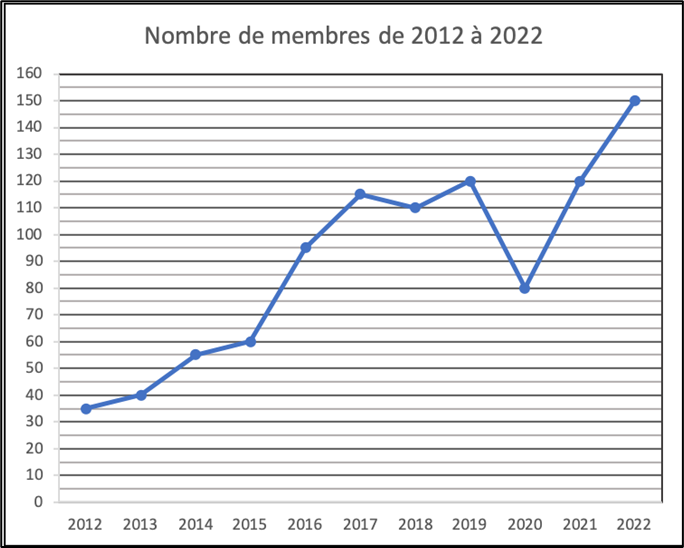
\includegraphics[width=\linewidth]{img/voitures.png}
        \columnbreak
        \begin{enumerate}[itemsep=1cm, after=\vspace*{1cm}]
            \item Cite deux années où le club a compté le même nombre de membres.
            \item En quelle année le nombre d'inscrits a-t-il le plus augmenté ?
            \item Est-il vrai que le nombre d'inscrits a doublé entre 2015 et 2019 ? Laisse ta démarche visible.
        \end{enumerate}
    \end{multicols}
\end{transferer}
%%%%%%%%%%%%%%%%%%%%%%%%%%%%%%%%%%%%%%%%%%%%%%%%%%
%%%%%%%%%%%%%%%%%%%%%%%%%%%%%%%%%%%%%%%%%%%%%%%%%%
\begin{transferer}[points=4]
    Voici le plan de deux salles de spectacle. Réponds aux questions.
    \begin{center}
        \includegraphics[width=.49\linewidth]{tikz/stockholm.tikz}
        \hfill
        \includegraphics[width=.49\linewidth]{tikz/berlin.tikz}
    \end{center}
    \begin{enumerate}[itemsep=1cm, after=\vspace*{3cm}]
        \item Exprime à l'aide d'une expression littérale le périmètre de la salle de Stockholm.
        \item Calcule l'aire de la salle de Berlin. Laisse tes étapes visibles.
    \end{enumerate}
\end{transferer}
%%%%%%%%%%%%%%%%%%%%%%%%%%%%%%%%%%%%%%%%%%%%%%%%%%
%%%%%%%%%%%%%%%%%%%%%%%%%%%%%%%%%%%%%%%%%%%%%%%%%%
\newpage
\begin{transferer}[points=4]
    Observe le pavage ci-dessous puis complète les égalités.

    \begin{minipage}{.5\linewidth}
        \includegraphics[width=\linewidth]{tikz/pavage.tikz}
    \end{minipage}
    \hfill
    \begin{minipage}{.45\linewidth}
        \begin{center}
            \begin{enumerate}[itemsep=.4cm]
                \item \(t_{\overrightarrow{NB}} (M)= \blank[width=1cm]{}\)
                \item \(S_H(A)=\blank[width=1cm]{}\)
                \item \(S_{WQ}(P)=\blank[width=1cm]{}\)
                \item \(t_{\overrightarrow{E\blank[width=1cm]{}}}(G)=L\)
                \item \(S_I(C)=\blank[width=1cm]{}\)
                \item \(t_{\overrightarrow{UJ}}(Q)=\blank[width=1cm]{}\)
                \item \(S_{MG}(A)=\blank[width=1cm]{}\)
                \item \(S_{P\blank[width=1cm]{}}(F)=R\)
            \end{enumerate}
        \end{center}
    \end{minipage}
\end{transferer}

\begin{appliquer}[points=1]
    Donne l'ensemble des diviseurs de 100.\vspace*{1cm}
\end{appliquer}

\begin{connaitre}[points=2]
    Écris :
    \begin{enumerate}[itemsep=1em]
        \item Deux nombres premiers entre eux :
        \item Deux multiples de 4 consécutifs :
        \item Un nombre multiple de 4 et de 7 :
        \item Trois nombres premiers :
    \end{enumerate}
\end{connaitre}

\begin{appliquer}[points=1]
    Décompose 360 en un produit de facteurs premiers.
\end{appliquer}
\end{document}
